% \documentclass[preprint]{sigchi}
\documentclass{sigchi}

\usepackage{fancyhdr}
\pagestyle{fancy}


\lhead{Three Month Report}
\rhead{2nd February 2015}

% Use this command to override the default ACM copyright statement (e.g. for preprints). 
% Consult the conference website for the camera-ready copyright statement.


% EXAMPLE BEGIN -- HOW TO OVERRIDE THE DEFAULT COPYRIGHT STRIP -- (July 22, 2013 - Paul Baumann)
\toappear{
% Permission to make digital or hard copies of all or part of this work for 
% personal or classroom use is 	granted without fee provided that copies are not made
% or distributed for profit or commercial advantage and that copies bear this notice
% and the full citation on the first page. Copyrights for components of this work 
% owned by others than ACM must be honored. Abstracting with credit is permitted. 
% To copy otherwise, or republish, to post on servers or to redistribute to lists, 
% requires prior specific permission and/or a fee. Request permissions 
% from permissions@acm.org. \\
% {\emph{CHI'14}}, April 26--May 1, 2014, Toronto, Canada. \\
% Copyright \copyright~2014 ACM ISBN/14/04...\$15.00. \\
% DOI string from ACM form confirmation
% {\emph{PhD 3 Month Report}}, 2 February 2015, Birmingham, UK.
}
% EXAMPLE END -- HOW TO OVERRIDE THE DEFAULT COPYRIGHT STRIP -- (July 22, 2013 - Paul Baumann)



% Arabic page numbers for submission. 
% Remove this line to eliminate page numbers for the camera ready copy
% \pagenumbering{arabic}


% Load basic packages
\usepackage{balance}  % to better equalize the last page
\usepackage{graphics} % for EPS, load graphicx instead
\usepackage{times}    % comment if you want LaTeX's default font
\usepackage{url}      % llt: nicely formatted URLs

% llt: Define a global style for URLs, rather that the default one
\makeatletter
\def\url@leostyle{%
  \@ifundefined{selectfont}{\def\UrlFont{\sf}}{\def\UrlFont{\small\bf\ttfamily}}}
\makeatother
\urlstyle{leo}


% To make various LaTeX processors do the right thing with page size.
\def\pprw{8.5in}
\def\pprh{11in}
\special{papersize=\pprw,\pprh}
\setlength{\paperwidth}{\pprw}
\setlength{\paperheight}{\pprh}
\setlength{\pdfpagewidth}{\pprw}
\setlength{\pdfpageheight}{\pprh}

% Make sure hyperref comes last of your loaded packages, 
% to give it a fighting chance of not being over-written, 
% since its job is to redefine many LaTeX commands.
\usepackage[pdftex]{hyperref}
\hypersetup{
pdftitle={SIGCHI Conference Proceedings Format},
pdfauthor={LaTeX},
pdfkeywords={SIGCHI, proceedings, archival format},
bookmarksnumbered,
pdfstartview={FitH},
colorlinks,
citecolor=black,
filecolor=black,
linkcolor=black,
urlcolor=black,
breaklinks=true,
}

% create a shortcut to typeset table headings
\newcommand\tabhead[1]{\small\textbf{#1}}


% End of preamble. Here it comes the document.
\begin{document}

\title{A Nonliner Dynamics Approach to Human Activity Recognition Using
Inertial Sensors}

\numberofauthors{3}
\author{
  \alignauthor P\'erez-Xochicale M. A.\\
    \affaddr{University of Birmingham}\\
%     \affaddr{Address}\\
     \email{perez.xochicale@gmail.com}\\
%     \vspace{2mm} \affaddr{PhD 3 Month Report \\2 February 2015}
%   \alignauthor 2nd Author Name\\
%     \affaddr{Affiliation}\\
%     \affaddr{Address}\\
%     \email{e-mail address}\\
%     \affaddr{Optional phone number}    
%   \alignauthor 3rd Author Name\\
%     \affaddr{Affiliation}\\
%     \affaddr{Address}\\
%     \email{e-mail address}\\
%     \affaddr{Optional phone number}
}

\maketitle

\begin{abstract}
The aim of the PhD is to gain understanding of concepts from nonlinear dynamics that 
can be used to extract features to identify complex activities involved in dance.
The research will contribute to the novel analysis and interpretation of data from 
inertial sensors and provide open source software and hardware to recognize activities 
in more realistic conditions. 
% The PhD has the potential to make a major 
% contribution to the field of human activity recognition.


% This three month report presents several challenges for Human Activity Recognition (HAR)
% as well as the state-of-the-art literature in motion caputure systems, machine learning 
% algorithms in HAR and human body analysis using nonlinear dynamics.
% It is also presented the proposed framework and timeline for the next six months
% of the PhD research.
% ,by which is hypothesided that 
% a proposal 
% in which indentifying complex activities involved in dance
% The aim of the PhD is focused on a full understanding of the 
% The current work concepts 
% from nonlinear dynamics that can be used 
% as a feature extraction for machine learning algorithms so as to provide 
% a robust HAR approach for real-time applications using inertial sensors.
% 
% We therefore hypothesize the current work has the potential
% to make major contribution to 

% This report is organised as follows: 
% % First, 
% the state-of-the-art in motion capture systems, machine learning approaches in HAR
% and human body analysis using nonlinear dynamics are presented in Section 2. 
% In the next section, the proposed framework and the workplan is presented.


\end{abstract}

\keywords{
  Human Activity Recognition; Body Sensor Networks; 
  Machine Learning Algorithms; Nonliner Dynamics.
}


\section{Introduction}

Human Activity Recognition (HAR) has been a challenging task \cite{Aggarwal2004}, 
since human body activity is complex and highly diverse \cite{Kim2010}.
HAR has many potential applications; for instance, these can be seen in personal 
assistants, surveillance, patient monitoring, sports analysis, dance activities, 
human-robot interaction and biometrics to mention but a few \cite{Aggarwal2011}. 
HAR has given several frameworks in recognizing primitive activities 
such as walking, jogging, cycling, jumping; nonetheless, little work has been been
done in identifying complex activities that for instance involve dance. 
Dance activities reflects the dancer's profile i.e., rhythmic sense, 
home country \cite{Iwai2011}, personality, biological features (i.e., genre and age),
dancing skills (i.e., fluency of the motion, adding erractical or additional movements,
coordination and turbulence in dance, steadynees of the rhythm, predictability of 
the motion) \cite{GrammerK.ElisabethOberzaucher2011}.
Recently, researchers in human body activity and gait recognition have proposed
the use of concepts from nonlinear dynamics (\textit{e.g.}
time-delay embedding theorem \cite{J.FrankS.Mannor2010,Sama2013}
and attractors in the state space \cite{Akiduki2013,Akiduki2014}) 
that have been proven to be an efficient approach 
for classification purposes as well as for indentification activities 
in real time in low-powered devices. 

Henceforth, the current PhD work is aimed to gain understanding of 
concepts from nonlinear dynamics that can be used to extract features and
to address the multiattribute classification problem that is involved 
in dance activities.

\subsection{Research Questions}
HAR deals with many issues which are
a) the different types of activities to recongnise,
b) the selection of motion capture system which should be unobtrusive and inexpensive,
c) the selection of algorithms for feature extraction and classification,
d) and the response time (offline or online) \cite{Lara2013}.
Yet, the chosen approach varies almost as greatly as the types of activities 
that have been recognized and types of sensor data that have been used 
\cite{Kim2010}. 
Additionally, HAR has many challenges that motivate our work 
to find new techniques in order to recognize activities in more realistic conditions. 
Therefore, finding appropriate methods for HAR is not only motivated by the 
fact that the motion capture system should be non-intrusive and easy-to-wear
but also that theoretical approach should be well suited for real-time applications.

To fullfil the previous-stated seatbacks, the following research questions will be addressed:

\begin{enumerate}
  \setlength{\itemsep}{0pt}
  \setlength{\parsep}{0pt}
  \item Which non-reported concepts from nonlinear dynamics could be use to obtain 
	another features for human body analysis?
  \item How can motion of the body parts (wrist, ankle, hips, shoulders, etc)
        be quantified so as to set features for the better HAR?
  \item Which axises among accelerometer, gyroscope and magnetometer 
	will provide the best information to identify complex activities?
  \item Which machine learning algorithm would be more suitable to identify complex 
    activities such as dancing.
%   \item Passive dynamic walking model has been used to investigate nonlinear gait 
% 	dynamic \cite{Kurz2007}. 
% 	Does the development of models for diffent human body activities 
% 	would be an accurate approach for real-time recognition?
%   \item Would be suitable to build models based on the reconstructed attractors 
% 	\cite{Nikulchev2013} for different human body activities in real-time 
% 	applications?
%   \item It has been reported that up to 50 human activities can be recongnized using 
% 	video based approached \cite{Reddy2012}.
% 	How many human body activities and with what accuracy can be recognized
% 	using the current proposal?
\end{enumerate}

% We therefore hyphotesise that this work has the potential to 
% make a major contribution to the human activity recogntion field
% 
% Thus, the aim of the PhD is focused on a full understanding 
% of the concepts from nonlinear dynamics that can be used 
% as a feature extraction for machine learning algorithms so as to provide 
% a robust HAR approach for real-time applications using inertial sensors.

% This three month report is organised as follows: First,
% the state-of-the-art in motion capture systems, machine learning approaches in HAR
% and human body analysis using nonlinear dynamics are reviewed in Section 2. Sencond, 
% the proposed framework and the workplan is presented in section 3.

\section{Previous Work}

% The central goal of the research proposal is focused on a full understanding of 
% concepts from nonlinear dynamics that can be used for human activity recognition 
% so as to provide a robust approach for real-time identification using inertial sensors.
% Thus, 
Reviews of motion capture systems, 
machine learning approaches in HAR and human body analysis using 
nonlinear dynamics are presented in the following sections.

% are presented. Additionally, 
% different approaches for HAR 
% that use concepts from nonlinear dynamics are reviewed. 

\subsection{Motion Capture Systems}
Motion capture systems can be chategorised into three approaches: 
vision-based \cite{Forsyth2005}; 
floor-sensor based
\cite{Paradiso1997,Steinhage2008,Aguilar2007,Wimmer2011,Yin2003,Moere2004,
Richardson2004,Srinivasan2005, Rangarajan2008,Visell2010, Rajalingham2010}
; and inertial-sensor based
\cite{Razak2012,Bamberg2008,Benocci2009,Xu2012,Holleczek2010}.
Although vision-based and floor-sensor based are rooted in non-intrusive 
motion capture systems, these are still required to be used into the space 
where users are constrained to move around.
On the other hand, wearable systems have been proven to be the least instrusive 
and easy-to-use sensors. However, the choosen approach for 
the motion capture system varies as greately as the 
types of activities that have been recognized 
and many other factors such as type of sensors, data connection protocol, obstrusiveness, 
recognition performance, energy consumption, flexibility, computational processing,
features, learning, and accuracy 
are considered for the performance of the motion capture system \cite{Lara2013}.

\subsection{Machine Learning Aproaches in HAR}
Much attention has also been given in recent years to use machine learning 
algorithms in HAR since the identification of activities entail a large number of 
attribute values and different transition points between activities;
to this end several approaches have been used i.e. 
Suppor Vector Machines \cite{J.FrankS.Mannor2010, Sama2013, Schuldt2004},
template matching \cite{Nguyen2009,Lin2007}, 
Hidden Markov Model 
\cite{Kohn2012,Niu2004,Chen2003,Bernardin2003,Eickeler1998,Chang2000},
Dynamic Time Warping \cite{Bautista2013,Boulgouris2004,Celebi2011},
Neural Networks \cite{Rosenblum1994,Ji2013,Modi2011,Boesnach2004},
and  most recently Dynamic Bayesian Networks \cite{Cuaya2013, Wang2014}, 
Emerging Patterns \cite{Tao2009, Kim2010},
Conditional Random Field  \cite{Wang2006} and
Skip Change Conditional Random Field \cite{Kim2010}. 
However, much research remains to be done to find suitable machine learning 
algorithms to identify complex activities that are presented in dance activities.


\subsection{Human Body Analysis Using Nonlinear Dynamics}

Recently, the use of intertial-based motion capture system in human body activity 
and gait recognition has been proposed the use of concepts from nonlinear dynamics 
that implements methods to obtain; for instance, the state space reconstruction,
determinism test, Lyapunov exponents and Poincar\'e maps.
These concepts have been proven to be efficient approaches to meet the computitional 
requirements for processing information in real time
\cite{J.FrankS.Mannor2010, Sama2013, Gouwanda2012,Perc2005, Akiduki2013,Akiduki2014}. 

Similarly, video-based approaches have been proven to present good results 
to recognize more complex human body activities such as the dextery of tennis players 
using attractors and fractal properties \cite{Yamamoto2000,Suzuki2013} 
, identification of dancing ballet, jumping, running, sitting and walking activities
using the attractors of the reconstructed state space, 
multivariate phase space reconstruction
and Maximal Lyapunov Exponent 
\cite{Ali2007,Basharat2009,Venkataraman2013}, and the recongnition of 
two-dimensional single-stroke patterns of 26 letters 
through modeling the attractor behaviors \cite{Ijspeert2013}. 

On the other hand, concepts from nonlinear dynamics also have been used to understand 
the behavior of human body activities for clinical applications, for instance
Vieten \emph{et al.} \cite{Vieten2013} quantify differences between gait patterns 
under constraints by approximating the time series data that underlying limit cycle 
attractors. 
Harbourne \emph{et al.} \cite{Harbourne2009} presented evidence 
to make diferentiation between health and nonhealth subjects and 
to identify difference between young and old people 
by analysing the changes in the attractor in the state space.
Zhang \textit{et al.} \cite{Zhang2010} demonstrated that the points of the 
Poincar\'e section are highly susceptible to noise; however, the use of power 
spectrum density analysis of the correlation coefficient demonstrate a relationship 
between $1/f$ noise and healthy subjects is very strong.
Buzzi \textit{et al.} \cite{Buzzi2003} demonstrated satisfactorily that elderly 
subjects increased the inability to compensate the natural stride-to-stride variations
by using the Lyapnov Exponent (LyE) and surrogate LyE (s-LyE).
Terrier \textit{et al.} \cite{Terrier2013} analysed and characterized the 
synchronization of steps with an auditory stimulus to evaluate gait stability 
and fall risk by using the maximum LyE.
It is important to mention that researchers in this area have been made 
a greater emphasis on the need for embedded software to make accessible 
tools for physical therapist.

\section{How will the PhD advance research?}

This PhD will extend the field of HAR in three signigicant ways.
First, by analysing the time-series of the inertial sensors as a nonlinear systems, 
the research will create novel analysis of these data.
Second, by builing a Body Sensor Network, the research will create a non-intrusive motion 
capture system as well as open source software which will be suitable for online activity 
recognition in a more realistic condition. 
Third, by applying different machine learning algorithms to classify the complex activitites 
involved in dance, the research will contribute to interpretation of the data so as
to evaluate the accuracy in different classifiers.
% and create novel machine algorithms.
% the reconstructed state space.
% the research applying concepts from nonlinear
% dynamics, the research will create nvel analysis  and interpretation of these
% data. The work has the potential to make a major contribution to 
% the field of human activy recogntion.

\section{Research Methods}
\subsection{Takens's Theorem}

In this work we follow the notation employed in \cite{Casdagli1991,Uzal2012}.
The purpose of the Takens's Theorem also knowns as time-delay embedding theorem 
is to reconstruct a $D-$dimensional manifold \textbf{M} $s(t)$ of an unknown dynamical 
system from time series $x(t)$ of that system. 
The time series is a sequence $x(t)=h(s(t))$, where $h: M \rightarrow \mathbb{R}^D$
is a measurement function on the unknown dynamical system, being $x(t)$ is observable.
The time delay reconstruction in $m$ dimensions with time delay $\tau$ is defined as:
$\overline{x}(t) = (x(t), x(t-\tau),...,x(t-(m-1)\tau))$ which defines a map
$\varPhi: M \rightarrow \mathbb{R}^m$ such that $\overline{x}(t) = \varPhi(s)$.
$\varPsi: \mathbb{R}^m \rightarrow \mathbb{R}^n$ is a further transpormation that
is considered as a more general transpormation in which for the 
current work we are applying the Principal
Component Analyis PCA algorithm (Figure \ref{fig:takens_theorem}).

\begin{figure}[htbp!] 
\centering    
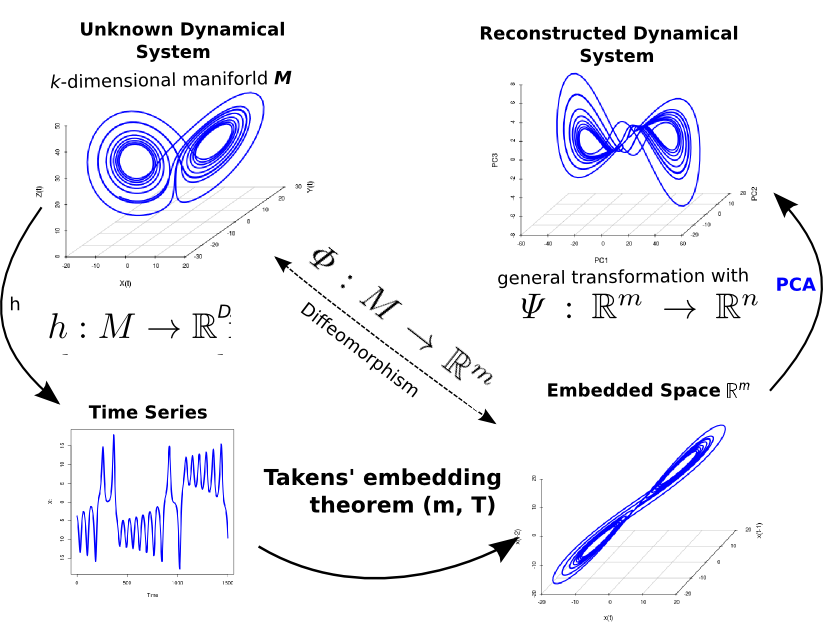
\includegraphics[width=0.45\textwidth]{takens_theorem_v3}
\caption[PA]{The reconstruction problem}
\label{fig:takens_theorem}
\end{figure}

Although the Takens's Theorem is well studied, there is still 
research to be done to find the optimal embedded parameters ($m$ and $\tau$) 
that largely depends on the application at hand \cite{J.FrankS.Mannor2010,Sama2013}.

% \subsection{Machine Learning Toolkits}
% As it has been said in the Section of Machine Learning Aproaches in HAR,
% there are many methods that can be used, however, there is 

\section{Current Progress}

\subsection{Body Sensor Network}
It has been proposed a Body Sensor Network (BSN) which has four Razor 
9DOF Inertial Measurements Units from sparkfun and its ARF7044 bluetooh modules 
from Adeunis. The data is collected at a sampling rate of 50 Hz by using a C++ class. 
Both hardware and software are under development and these work on 
GNU$\backslash$Linux (Ubuntu 12.04 32 bits distribution).

\subsection{Preliminary Experiments}
By establishing a basic latin dance foot pattern as the human activity to characterize,
the user has been asked to perform this activity in repetitive times. 
The inertial sensor was worn in the right ankle.
We then collected the time series for the roll euler angle 
(Figure \ref{fig:example} (a)). 
The embedding parameters for the the time-delay embedding reconstruction 
are $m=30$, $\tau=3$. Finally, we transform the reconstructed state space
by using the PCA algorithm and plot the first three components
(Figure \ref{fig:example} (b)).
\begin{figure}[htbp!] 
\centering    
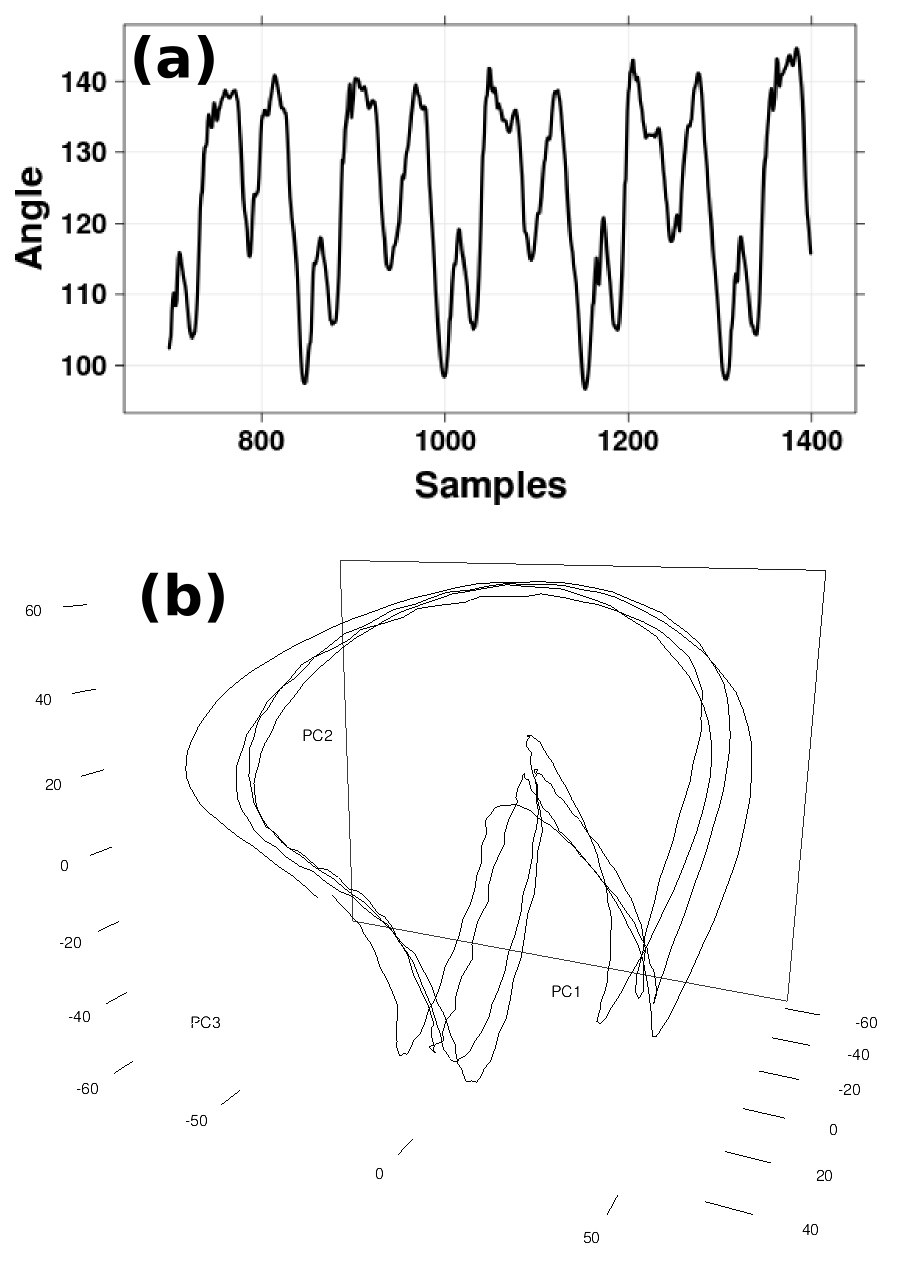
\includegraphics[width=0.4\textwidth]{experiments_v0}
\caption[PA]{(a) Time series for the roll euler angle, (b) 
First three components of PCA of the reconstructed state space with $m=30$, $\tau=3$.}
\label{fig:example}
\end{figure}
We are analysing the time series of different sensor position as well as 
the use of different components so as to to obtain obtimal embedded parameters
for the reconstructed state space by using Cao's method \cite{Cao1997}.


\section{6 month plan}
The proposed framework is divided into five modules (Figure \ref{fig:proposedapproach}): 
1) Data acquistion using a Bluetooth body sensor network with Inertial Measurement Units, 
2) Reconstruction of the state space with a C++ class, 
3) nonlinear measuraments and feature extractions by means of Principal Component
Analysis, 
4) classification using state-of-the-art multiatribute machine learning algorithms, 
and  5) application(s) such as dancing. 
Based on the proposed framework, 
tasks for the following 6 months are planned as follows:
\begin{itemize}
% [noitemsep,topsep=0pt,parsep=0pt,partopsep=0pt]
%  \item T1: 5 curses will be taken and they will be suggested by the doctoral committee.
\item T1 [February]: Review of state-of-the-art machine learning methods 
for human activity recognition using wearable sensors.
\item T2 [March]: Define the human activity experiment and recruit subjects 
to collect data so as to test the proposed PhD framework by means of a suitable
machine learning algorithm.
\item T4 [April]: Write and submit a paper in the 19th annual International Symposium
on Wearable Computers (Full/Note Paper Due: 10 April)
\item T5 [May-June]: Update the hardware of the body sensor network by using
Bluetooth low energy devices.  
\item T6 [May-June]: Update the open source sofware library for the body sensor
network.
\item T6 [July]: Write the 9th month report and create a publication
plan for the next year.
\end{itemize}

\begin{figure}[htbp!] 
\centering    
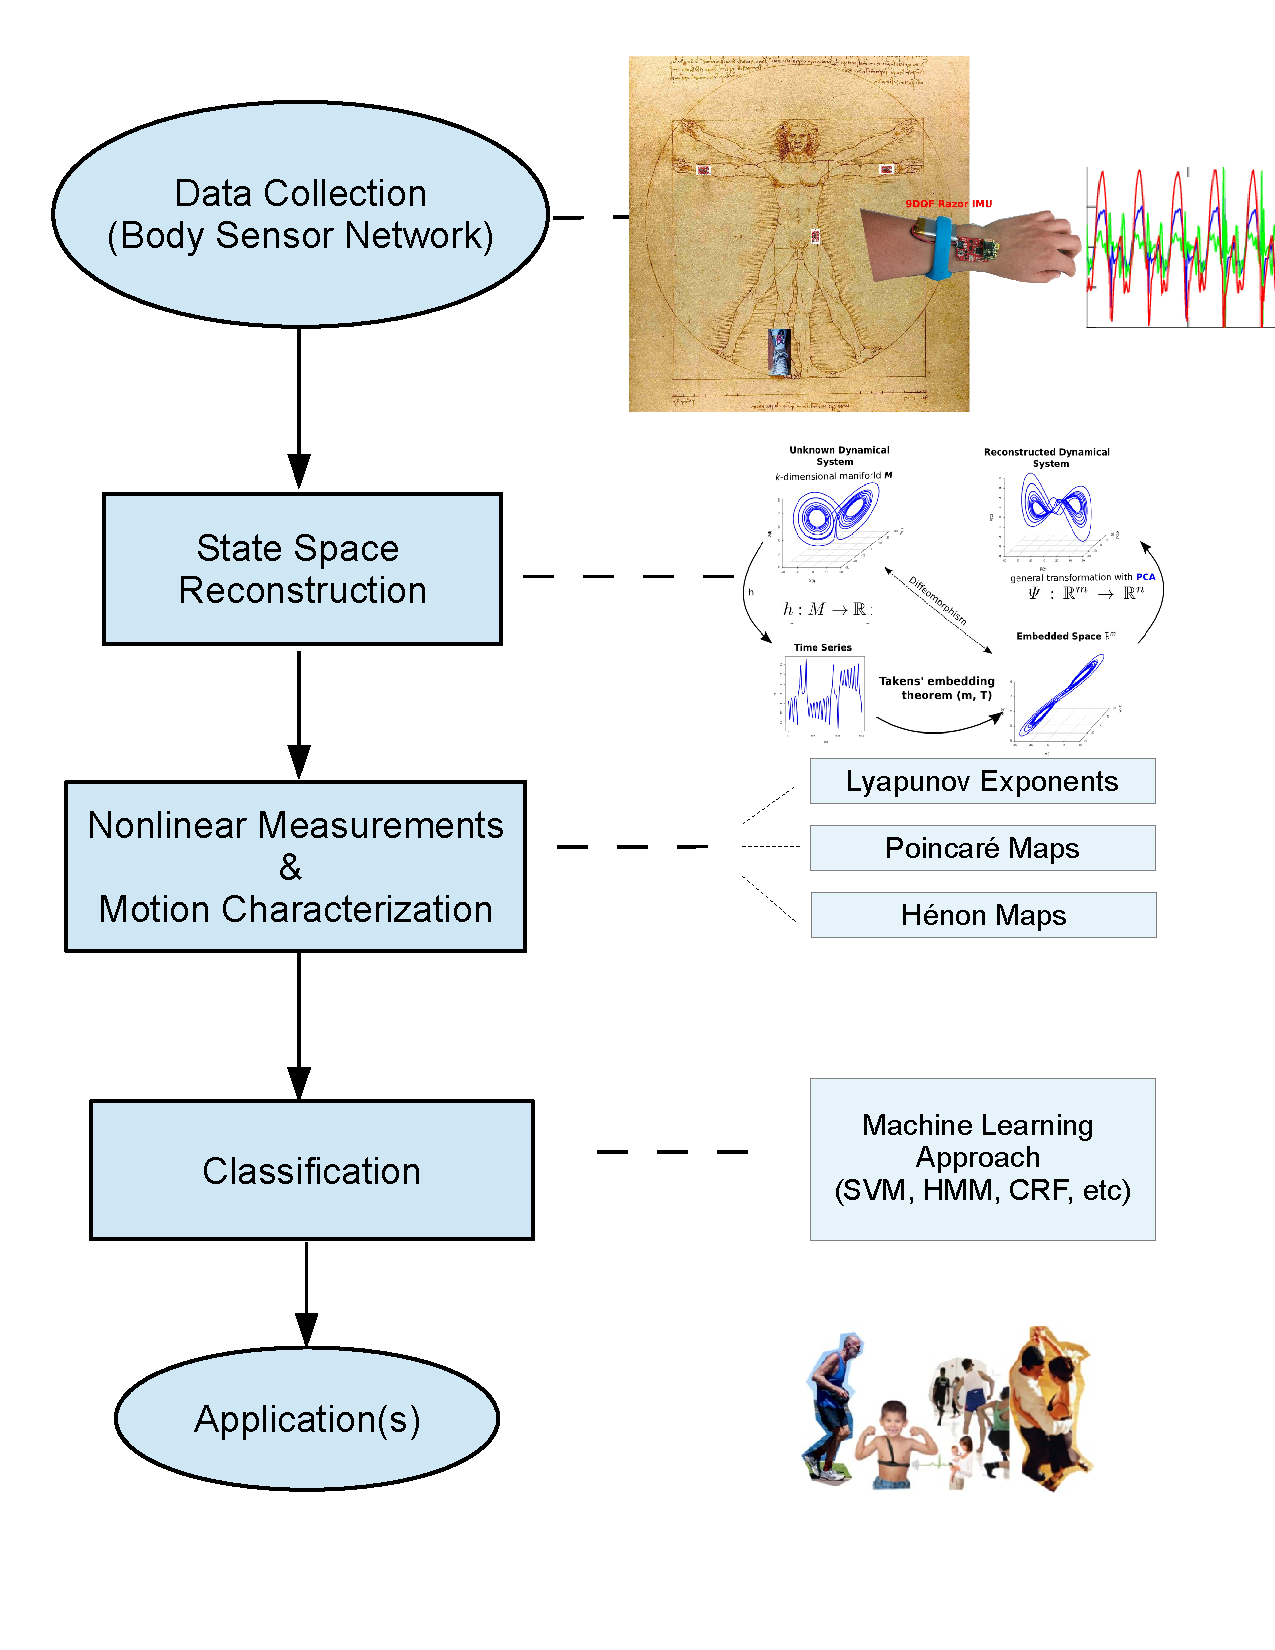
\includegraphics[width=0.5\textwidth]{proposedapproach_v1}
\caption[PA]{PhD Framework}
\label{fig:proposedapproach}
\end{figure}

% It is important that you write for the SIGCHI audience.  Please read
% previous years' Proceedings to understand the writing style and
% conventions that successful authors have used.  It is particularly
% important that you state clearly what you have done, not merely what
% you plan to do, and explain how your work is different from previously
% published work, i.e., what is the unique contribution that your work
% makes to the field?  Please consider what the reader will learn from
% your submission, and how they will find your work useful.  If you
% write with these questions in mind, your work is more likely to be
% successful, both in being accepted into the Conference, and in
% influencing the work of our field.

\section{Acknowledgments}
The author acknowledge support from Mexico's National Council 
for Science and Technology, CONACyT, to pursue doctoral research at the 
University of Birmingham.

% Balancing columns in a ref list is a bit of a pain because you
% either use a hack like flushend or balance, or manually insert
% a column break.  http://www.tex.ac.uk/cgi-bin/texfaq2html?label=balance
% multicols doesn't work because we're already in two-column mode,
% and flushend isn't awesome, so I choose balance.  See this
% for more info: http://cs.brown.edu/system/software/latex/doc/balance.pdf
%
% Note that in a perfect world balance wants to be in the first
% column of the last page.
%
% If balance doesn't work for you, you can remove that and
% hard-code a column break into the bbl file right before you
% submit:
%
% http://stackoverflow.com/questions/2149854/how-to-manually-equalize-columns-
% in-an-ieee-paper-if-using-bibtex


\bibliographystyle{acm-sigchi}

% \bibliography{sample}
\bibliography{References/references} % Path to your references.bib file

\end{document}
